% Chapter 6

\chapter{Z-Wave} % Main chapter title

\label{Chapter6} % For referencing the chapter elsewhere, use \ref{Chapter6}

\lhead{Chapter 6. \emph{Z-Wave}} % This is for the header on each page - perhaps a shortened title
Homelive use a new Smart Home communication technology -- Z-Wave. TR-069 Client should be able to retrieve the data in Luup and synchronise with TR-069 data model and ACS.

\begin{figure}[htbp]
	\centering
		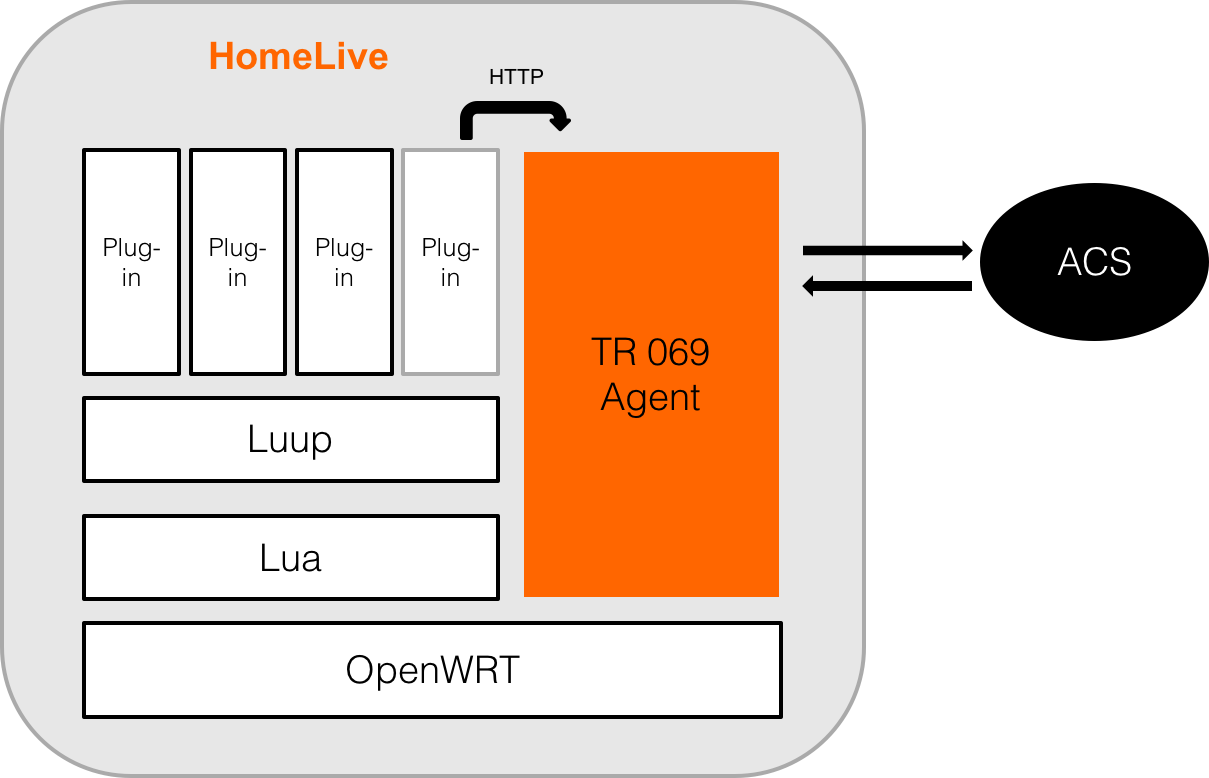
\includegraphics[width=12cm]{Figures/homelivestructure.png}
	\caption[Homelive Structure]{Homelive Structure}
	\label{fig:homelive}
\end{figure}

%----------------------------------------------------------------------------------------
\section{Protocol Z-Wave}
Z-Wave is a standardized protocol for automation wireless habitat solution. It was designed by the Danish company \textit{Zen-Sys} which was later bought by the US company \textit{Sigma Designs} in 2008. \textit{Sigma Designs} and the Japanese company Mitsumi provides the Z-Wave chips.

Z-Wave equipment manufacturers are gathered in the Z-Wave Alliance. Founded in 2005, it promotes the protocol and ensures interoperability between devices. Interoperability is true on two levels: Radio layer and application layer. Certified equipment receive the Z-Wave logo (see \fref{fig:zwavelogo}). More than three hundred companies have since joined this alliance.

\begin{figure}[htbp]
	\centering
		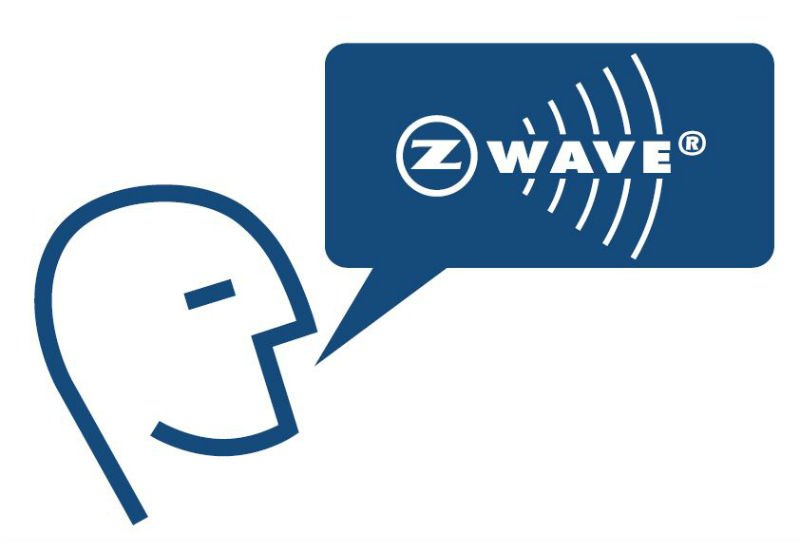
\includegraphics[width=8cm]{Figures/zwavelogo.jpg}
	\caption[Z-Wave Protocol Logo]{Z-Wave Protocol Logo}
	\label{fig:zwavelogo}
\end{figure}

The Z-Wave radio protocol is optimized to communicate with low bandwidth (between 9 and 40 kbps) and applied on stand-alone power supply or mains-powered, as opposed to Wi-Fi, which is intended for exchanges broadband.

\begin{center}
  \begin{tabular}{@{} cccc @{}}
    \toprule
    Requirements\textbackslash Protocol & \textbf{Z-Wave} & \textbf{Zigbee} & \textbf{En-Ocean} \\*
    \midrule
    \textbf{Reliability} & Yes & Yes & No \\
    \textbf{Security} & Yes & Yes & No \\
    \textbf{Radio waves Reduction} & Yes & Yes & Yes \\
    \textbf{Simplicity of use} & Yes & - & No \\
    \textbf{Better pricing} & Not yet & Not yet & No \\
    \textbf{Capitalization} & Yes & - & Yes \\
    \textbf{Interoperability} & Yes & No & Yes \\
    \bottomrule
  \end{tabular}
%	\caption[Homelive Box of Orange]{Homelive Box of Orange}
\end{center}
\begin{figure}[htbp]
	\centering
		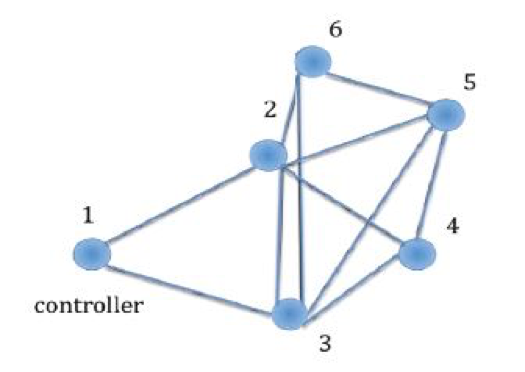
\includegraphics[width=8cm]{Figures/zwavenetwork.png}
	\caption[A Z-Wave Mesh Network Example]{A Z-Wave Mesh Network Example}
	\label{fig:zwavenetwork}
\end{figure}

%----------------------------------------------------------------------------------------
\section{Data Model Z-Wave}
Orange has defined its own Z-Wave data model, which is divided into three parts:
\begin{itemize}
  \item The part \textit{Z-Wave Network} defines the network topology
  \item The part \textit{Z-Wave Structure} defines the set of information that can be recovered on the Z-Wave network to identify the devices.
  \item The part \textit{Z-Wave Device} contains architecture and device configuration.
\end{itemize}

\begin{figure}[htbp]
	\centering
		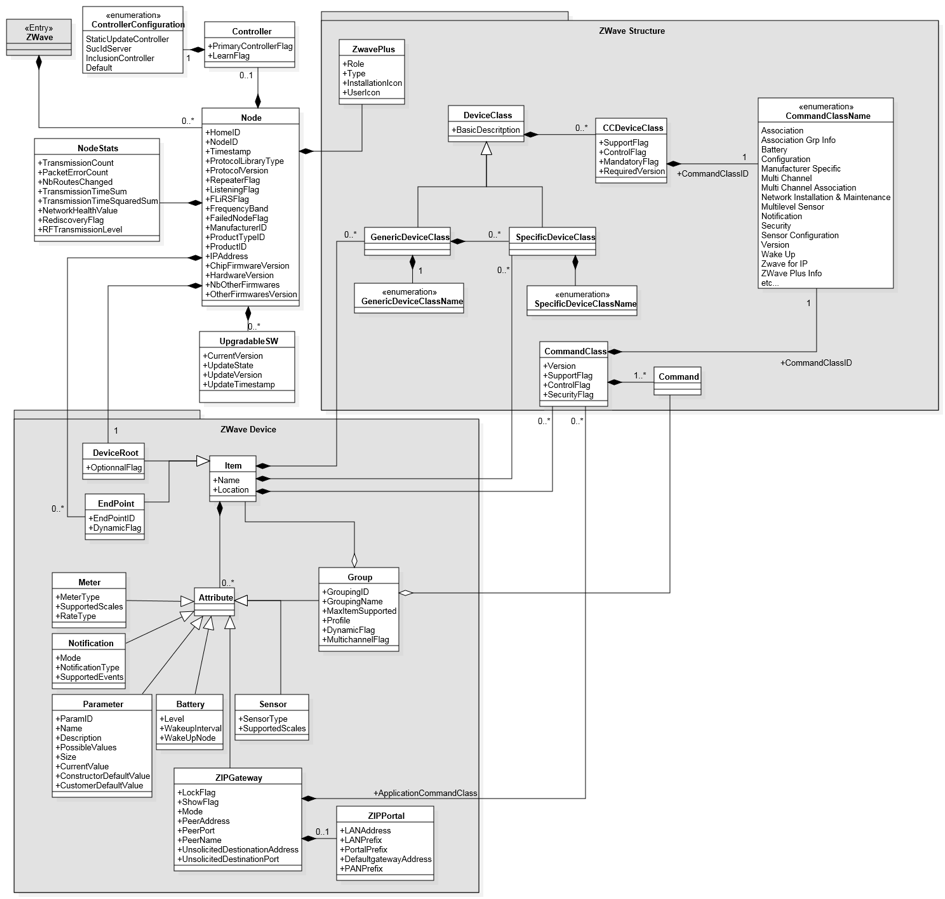
\includegraphics[width=14.5cm]{Figures/datamodel.png}
	\caption[Z-Wave Node Data Model]{Z-Wave Node Data Model}
	\label{fig:zwavedatamodel}
\end{figure}
%----------------------------------------------------------------------------------------
\section{Update Z-Wave in TR-069}
In order to retrieve the Z-Wave data from the Homelive Box, a http request to Homelive firmware can return a file(JSON or XML) which contains all the parameters that generated from lower layer. Then we should write a program to perser the file and save it in the TR-069 Client database.

\subsection{HTTP Request}
In addition to sending requests using standard UPnP, we can also do most things using a simple HTTP requests. Use the built-in URL data_request, and pass the following on the URL: \url{http://ip_address:3480/data_request?id=user_data&output_format=xml}.

This returns the configuration data for Vera, which is a list of all devices and the UPnP variables which are persisted between resets as well as rooms, names, and other data the user sets as part of the configuration.

In our case, we should retrieve the data of \textit{status}, so we change \textit{user_data} to \textit{status}. The hhtp request is been called in the Homelive, so we can replace it with the local address: \url{http://127.0.0.1/}. And in consideration of parser, we set the output format to \textit{JSON}. The request url become:\\
\url{http://127.0.0.1:3480/data_request?id=status&output_format=json}

We can call this http request by using the API already provided in TR-069 Client:
\begin{lstlisting}[mathescape]
    int DM_HttpGetFile(IN httpGetFileDataType * httpGetFileDataPtr)
\end{lstlisting}

After this, we will have the JSON file in format of Luup data model, the next step is to parse the file.

\subsection{JSON Parser}
JSON parser is not a default library of language C, so we have to find a JSON parser. Fortunately, in the Luup firmware, there is a JSON parser library already included, which is \textit{json-c}. My program is based on \textit{json-c} library and use a iterative strcture to parse the JSON file we retrieved from Luup( See Appendices 2).

After parse the JSON file, we will have a huge name\textbackslash value pairs, a two-dimension table is declred to saved them in buffer with dynamic memory management.

The next step is to find the correspondance between Z-Wave data model and Luup data model.

\subsection{Simple file Storage System}
TR-069 Client use simple file storage system as its data base. The structure is as following:

\begin{figure}[htbp]
	\centering
		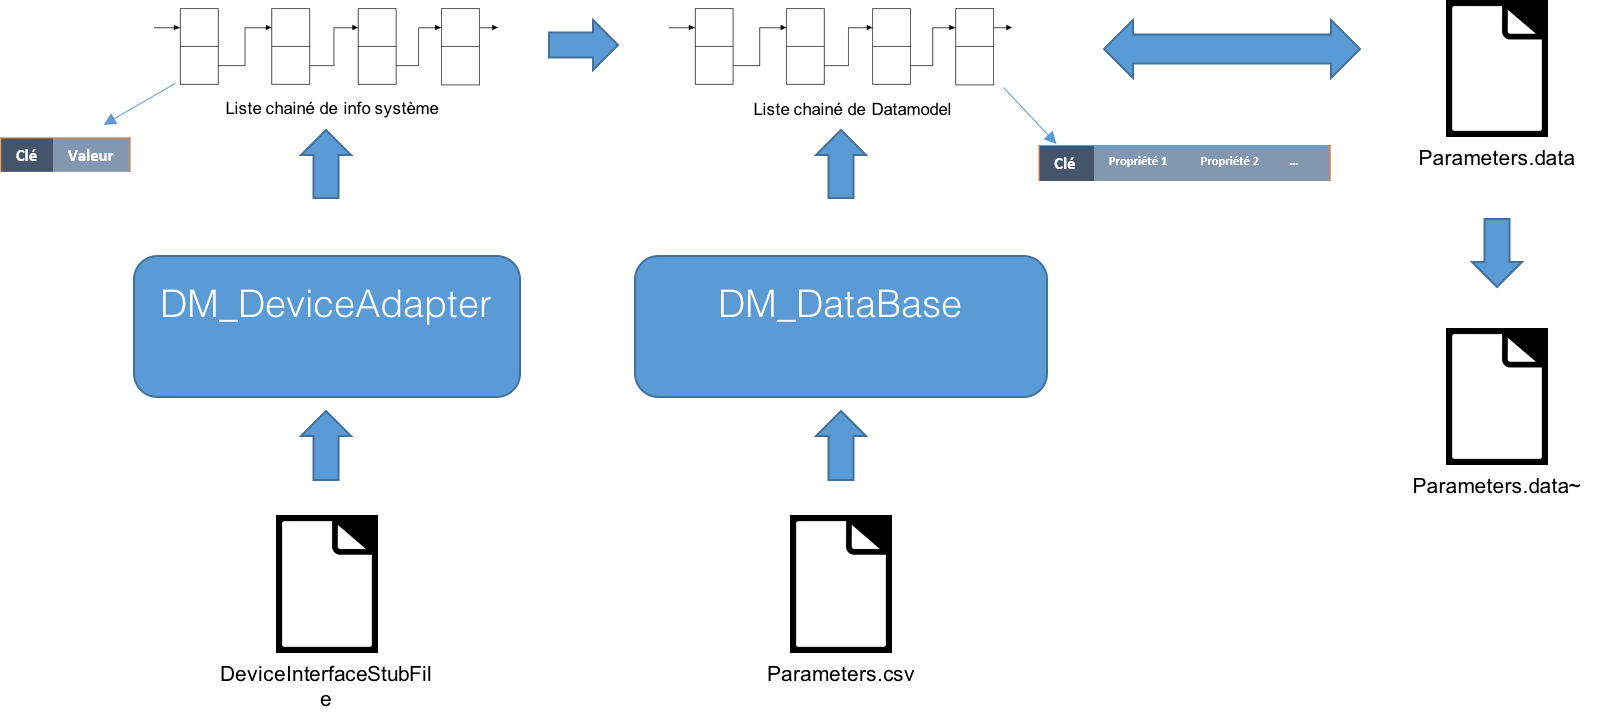
\includegraphics[width=14.5cm]{Figures/database}
	\caption[TR-069 Simple File Storage System]{TR-069 Simple File Storage System}
	\label{fig:database}
\end{figure}

When the program starts, there are two modules are in charge of manage the database. First is the module \textit{DM\_ DeviceAdapter}, it reads the configuration file \textit{DeviceInterfaceStubFile}, which contains the system parameters(Manufacturer, ProductClass, SerialNumber, etc..), and it will create a linked list to store the name\textbackslash value pairs.

After that, module \textit{DM\_ Database} will read the data model file \textit{parameters.csv} and build a linked list from it. In the \textit{parameters.csv}, there are name\textbackslash value of the data model and also 10 property(Datatype, Writable, Notification type, etc..). When finish building the long linked list, it will read the value from the short linked list(\textit{DeviceInterfaceStubFile}) and copy them into the long linked list.

In the runtime, a file called \textit{parameters.data} will be created, and TR-069 will store all the data model in this runtime file in format of CSV(Comma-separated values) as the storage base.

The backup file is called \textit{parameters.data\~{}}, before every modification made to datamodel, the \textit{parameters.data} will save all the information into \textit{parameters.data\~{}} as a backup and update its own value.


\subsection{Synchronization Data model Luup and Z-Wave}

The data model of Luup and Z-Wave have diifferent in approach but equally contains the data we need. For each data in Z-wave data model, we should find the correspondance in Luup data model. For example, in Luup there is a data called \textit{ZWave.devices.\{i\}.states.15.variable WakeupInterval}, the correspondance we found in Z-Wave is \textit{Device.Zwave.Interface.\{i\}.WakeUpInterval}. To synchronize the two data model, the value of \textit{WakeInterval} in Luup should be given to Z-Wave \textit{WakeInterval}. We have studied 100 paramenters in Z-wave, and there are 27 are directly accessible from Luup data model, 26 can be caculated from Luup data model. For instance, the translation is finished for those all.
